\section{The pseudo-pilot paradigm}
One of the aspects of ATC training involves the \textbf{simulation} of training scenarios.

Current training sessions for ATC consist of two individuals that communicate with each other \cite{eurocontrol:remote-piloting-2021}.
The first and most obvious one is the aspiring ATC in training, that communicates their instructions to solve the initial situation of the aforementioned training scenario.

Our focus is centered in the second individual: the \textbf{pseudo-pilot}. They are in charge
of executing the instructions the aspiring ATC communicated using scenario simulation tools.

As we have already mentioned, the main case of use of a pseudo-pilot is \textbf{ATC training}.
Nevertheless, we have recently seen a rising tendency to use it in other contexts, such as
the validation of novel techniques for their use in real ATC. A pseudo-pilot is the \textit{stand-in pilot},
listening, executing and responding to the ATC's instructions. Furthermore, they may participate
by simulating multiple aircrafts at the same time.

Generally speaking, every conventional pseudo-pilot system follows a working schema like the one described in
Figure~\ref{fig:pseudopiloto-convencional}

\begin{figure}[htbp]
	\centering
	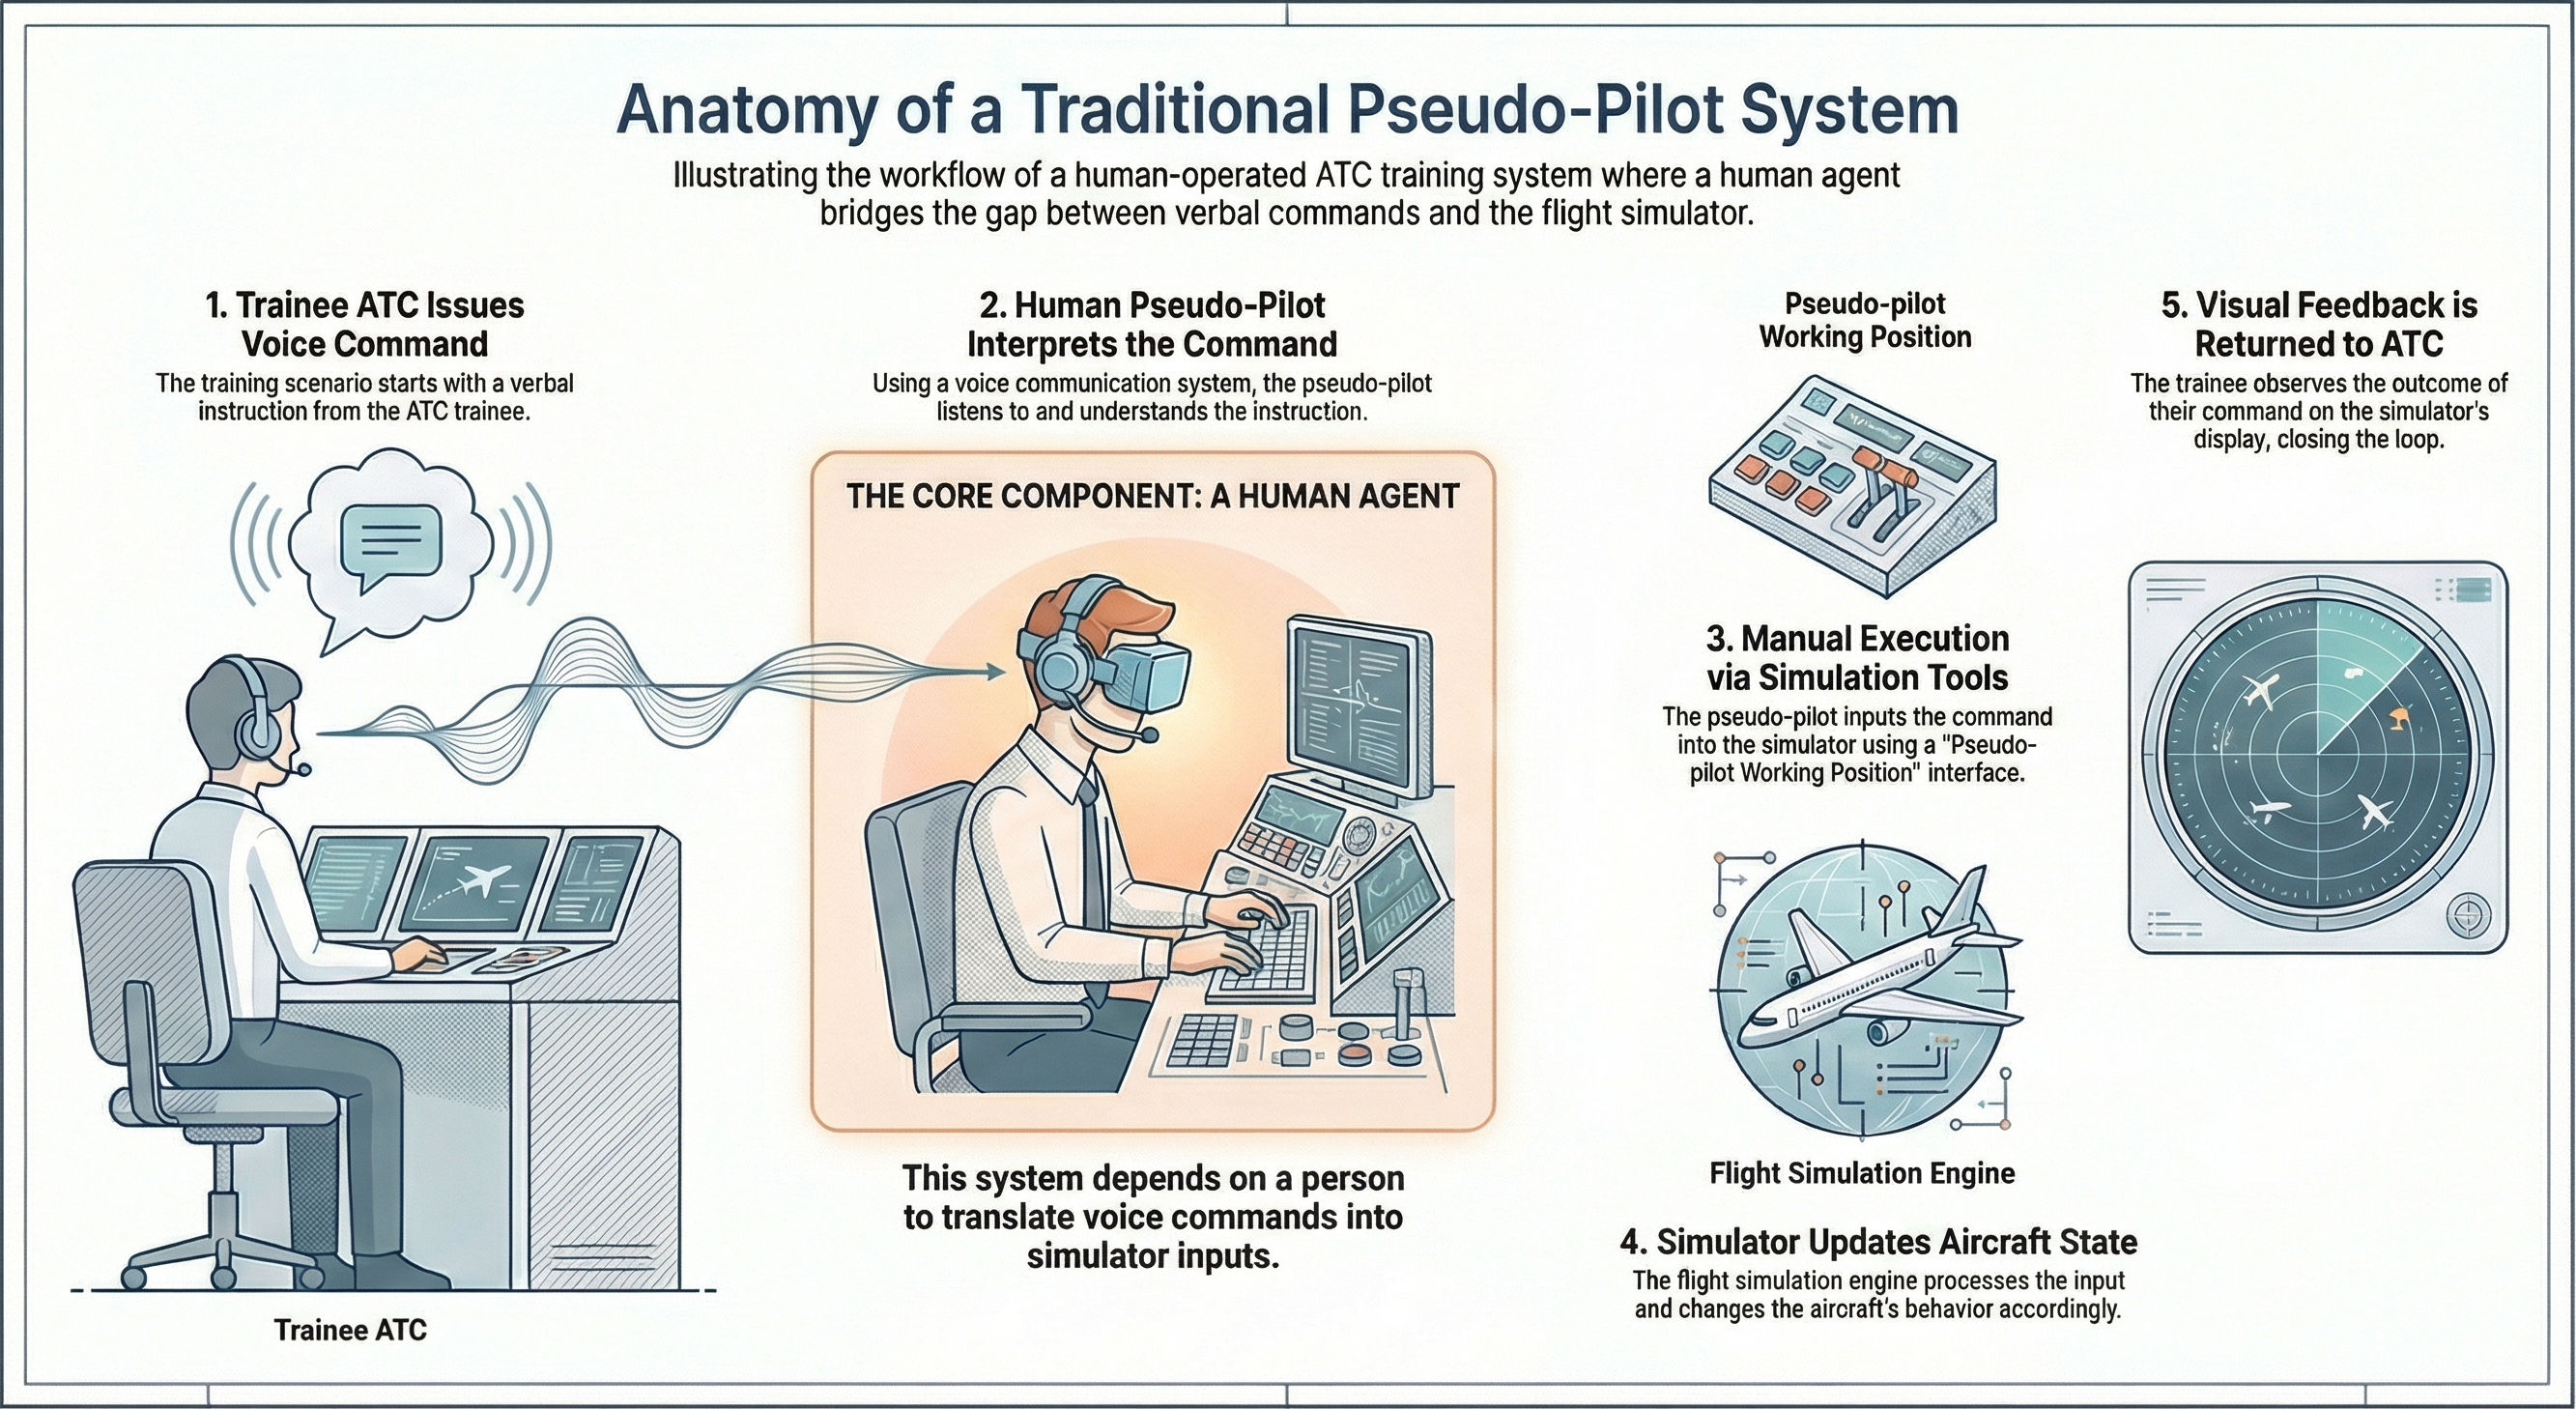
\includegraphics[width=1.1\linewidth]{assets/conventional-atc-diagram/unnamed.png}
	\caption{Schema of a conventional pseudopilot. The ATC emits instructions via voice communication channels and the pseudopilot executes them in the simulator. Finally, the simulation framework returns the feedback to the aspiring ATC.}
	\label{fig:pseudopiloto-convencional}
\end{figure}

A traditional pseudo-pilot typically includes a \textbf{Pseudo-pilot working position} which includes all pseudo-piloting tools. It's an accessible interface that allows users to control one or more aircrafts simultaneously, as well as edit the flight plans or other aspects of the simulation.

A Voice Communication System is also in place, allowing the pseudo-pilot to communicate with the trainee ATC using realistic aviation phraseology. Lastly, the \textbf{traffic generation software} generates traffic and complex situations automatically for their resolution by the ATC.

\section{Commercial State of the Art}

In order to understand the context in which our proposal makes a difference, it is crucial to comprehend the current status of the pseudo-piloting industry.
In more broad terms, we need to understand what the industry currently offers regarding ATC training. These systems define the industry standard and the tools that are used
today by human pseudo-pilots. Table~\ref{tab:simuladores_pp} offers a comparative view of these tools.

\begin{center}
	\begin{longtable}{>{\raggedright\arraybackslash}p{3.0cm}|>{\raggedright\arraybackslash}p{3.0cm}|>{\raggedright\arraybackslash}p{3.0cm}|>{\raggedright\arraybackslash}p{4.5cm}}
		\caption{Pseudo-pilot simulators summary}
		\label{tab:simuladores_pp}
		\\
		\toprule
		\textbf{Simulator (Provider)} & \textbf{Primary focus}                      & \textbf{Pseudo-pilot module}        & \textbf{Characteristics}                                                                                      \\
		\midrule
		\endfirsthead
		\multicolumn{4}{c}%
		{{\bfseries \tablename\ \thetable{} -- Pseudo-pilot simulators summary (Continued)}}                                                                                                                                              \\
		\toprule
		\textbf{Simulator (Provider)} & \textbf{Primary focus}                      & \textbf{Pseudo-pilot module}        & \textbf{Characteristics}                                                                                      \\
		\midrule
		\endhead
		\bottomrule
		\endfoot
		\bottomrule
		\endlastfoot

		ESCAPE (Eurocontrol)          & Training and Investigation                  & PWP                                 & Simultaneous control of multiple aircrafts. Advanced radar simulator.                                         \\
		\midrule
		BEST (MicroNav)               & Industry Standard                           & Integrated                          & \textbf{3D and 2D} simulation of aircrafts and \textbf{atmospheric conditions}.                               \\
		\midrule
		CSSOFT ATC Simulator (CSSOFT) & Step minimizing                             & Designed to \textbf{minimize steps} & Allows \textbf{as many flights as possible}. Advanced \textbf{syntax resilience} (minimizes operator errors). \\
		\midrule
		ATCTrSim (HAVELSAN)           & Training                                    & Intuitive and accessible UI         & Prioritizes \textbf{ease of use} for pseudo-piloting in training scenarios.                                   \\
		\midrule
		MaxSim (ADACEL)               & Complete ATC Simulation                     & \textbf{PWP}                        & Simulations use \textbf{real airports}.                                                                       \\
		\midrule
		Indra Simulator (Indra)       & Allows tower, approach and en-route control & \textbf{PWP}                        & 2D and 3D training. Multi-scenario interface.                                                                 \\
		\midrule
		SERA (ASTi)                   & Realistic communications                    & \textbf{Artificial Intelligence}    & Utilizes AI systems for traffic management within the simulator and phraseology reinforcement.                \\
	\end{longtable}
\end{center}

As we can see, solutions focus mainly on the features of each simulation software (2D and 3D, real airport usage, unlimited simultaneous flights...). The dominating paradigm in the industry revolves around the Pseudopilot Working Position. Tools like ESCAPE, MaxSim, or Indra's simulator are, essentially, advanced human interfaces that serve the purpose of providing a comfortable and realistic ATC training interface.
Even more modern AI-using tools like SERA apply it to manage communications, and not for the execution of the ATC instructions. This Commercial State of the Art analysis shows that the current industry depends on a human agent for command execution. None of these platforms offers the ideal execution by voice, essentially removing the
need for a human pseudopilot. This hints at the opportunity of the integration we propose.

\section{Research}

Although commercial solutions have not made any approaches that would resemble our proposal, the scientific literature has made some advances in the task of the pseudo-pilot automatization.

The idea of a completely autonomous pseudo-pilot system is not entirely novel. In 2005, Bolczak et al. \cite{bolczak2005accommodating} already proposed a proof of concept that integrated primitive ASR and TTS modules.
This early work was crucial, as it demonstrated a theoretical viability in automatizing the pseudo-pilot tasks completely. It did not become a standard due to the technical limitations of its time.

Recently, advances in the technologies used in \cite{bolczak2005accommodating} have caused a resurgence in the interest to automatize the pseudo-pilot. Lin et al. \cite{LinEtAl} propose the start of a more modular approach, where we firstly focus on
response generation for a pseudopilot. This would cause the human pseudo-pilot to only have to fulfill the ATC's instructions onto the flight simulation interface.

Later research by Zuluaga-Gomez et al.~\cite{Zuluaga-Gomez2023Virtual} provides a proof of concept that shows the automatization of the pseudo-pilot replies is possible. This means the pseudo-pilot would need to do less work, but it doesn't quite automate the full process. This begins to close the gap between the full automatization and the current state of the commercial systems.

With the aforementioned in mind, we have arrived at the model described by Figure~\ref{fig:pseudopiloto-respuesta-convencional}
\begin{figure}[htbp]
	\centering
	\includegraphics[width=1\textwidth]{assets/diagram_semiautomated/semiauto.png}
	\caption{Semi-automated schema proposed for the pseudo-piloting process. This integrates a supervised response module.}
	\label{fig:pseudopiloto-respuesta-convencional}
\end{figure}

This begins to close the gap between the full automatization and the current state of commercial systems.

The current SOTA is moving towards a paradigm that fully automates this system. Our proposal directly aligns with the direction in which the research is going, proposing a way to close the loop by directing instructions to a \textbf{Flightgear simulation interface}.